\section{Une étude de cas : Cholesky}\label{sec:contribs:apps:cholesky}

Afin de mettre en application nos analyses nous avons choisi comme cas d'étude une application d'algèbre linéaire populaire et bien connue : la factorisation de Cholesky.
Une manière standard de paralléliser les applications d'algèbre linéaire est de découper le problème en l'appliquant à différentes sous parties (ou \emph{blocs}) des matrices.

Nous allons étudier en détails l'algorithme de Cholesky par bloc, voir quelles sont ses parties critiques et leurs comportements, et nous allons également voir comment nous avons pu améliorer son exécution.


\subsection{Description générale}

La factorisation de Cholesky a pour but de résoudre l'équation suivante :

$$ A = L*L^T$$

Où $A$ est une matrice symétrique définie positive de nombre réels, et $L$ est l'inconnue, une matrice triangulaire inférieure.

Pour paralléliser la résolution de cette équation, on va découper la matrice $A$ par bloc, et appliquer un algorithme de Cholesky par bloc.
On peut donc caractériser une factorisation de Cholesky par sa taille de bloc et sa largeur en nombre de blocs.

L'algorithme de résolution par bloc repose sur quatre algorithmes basiques d'algèbre linéaire tirés des \emph{BLAS} - \emph{Basic Linear Algebra Subprograms} - décrit ci-dessous~:


\paragraph{\potrfcolor{POTRF(A)}}

Ce noyau effectue la factorisation de Cholesky de base sur une matrice $A$.

\paragraph{\trsmcolor{TRSM(A, B)}}

Ce noyau effectue l'opération suivante~: $A*X = B$, où $A$ est une matrice triangulaire, et $B$ une matrice générique. $B$ est écrasée par la matrice solution $X$.

\paragraph{\syrkcolor{SYRK(A, C)}}

Ce noyau effectue l'opération suivante~: $C = A*A' + C$, où $A$ est une matrice générique, et $C$ est une matrice symétrique.

\paragraph{\gemmcolor{GEMM(A, B, C)}}

Ce noyau effectue une multiplication de matrices génériques, définie de la manière suivante~: $C = A*B + C$, où $A$, $B$, et $C$ sont des matrices génériques.

\begin{figure}[h]
  \centering
  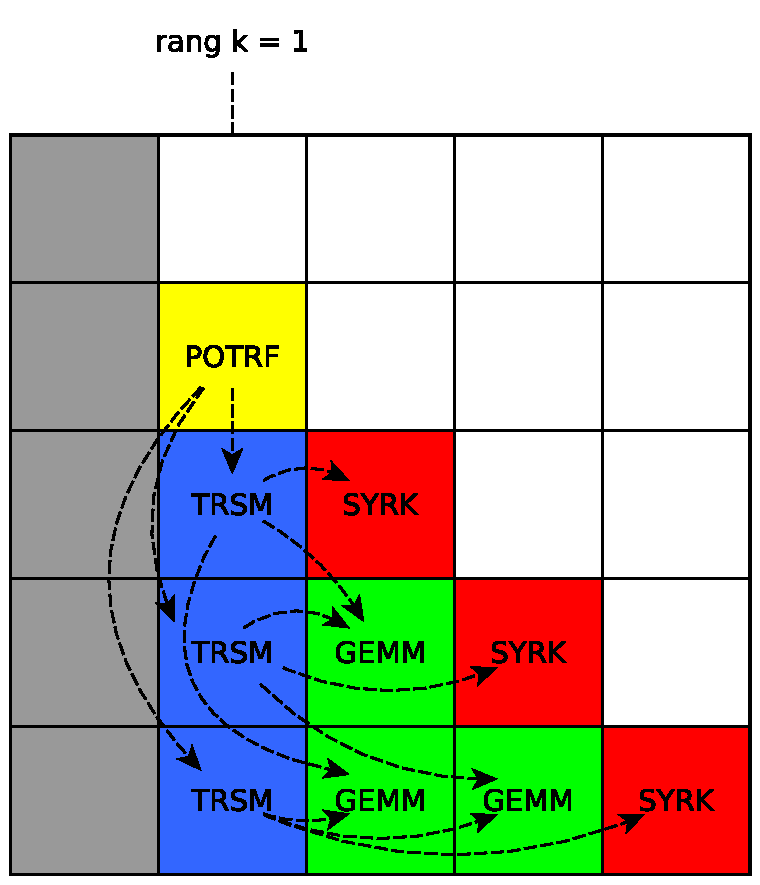
\includegraphics[width=0.6\textwidth]{cholesky-rank-update}
  \caption{Itération du rang k de la factorisation de Cholesky}\label{fig:contribs:apps:cholesky:rank-update}
\end{figure}

\paragraph{L'algorithme par bloc}

L'algorithme peut se formuler de la manière suivante~:

\begin{lstlisting}[language=c++]
for (int k = 0; k < n_blocs; k++) {
  DPOTRF(A(k, k));

  for (int m = k+1; m < n_blocs; m++) {
    DTRSM(A(k, k), A(k, m));

    for (int m = k+1; m < n_blocs; m++) {
      DSYRK(A(k, m), A(k, k));

      for (int n = k+1; n < m; n++) {
        DGEMM(A(k, n), A(k, m), A(n, m));
      }
    }
  }
}
\end{lstlisting}

Pour permettre de mieux représenter l'algorithme, les opérations se produisant sur chaque bloc de la matrice au rang |k| sont illustrées sur la figure~\ref{fig:contribs:apps:cholesky:rank-update}


À chaque itération, un \potrf est d'abord effectué sur le bloc diagonal de l'itération. Les blocs de la colonne sont ensuite mis à jour via des \trsm, à la suite desquels les autres blocs restant peuvent être mis à jour par des \gemm (ou \syrk pour les blocs diagonaux).
Le parallélisme de l'algorithme est donc principalement libéré par les \potrf ainsi que les \trsm.

Cela peut être illustré par la Figure~\ref{fig:contribs:apps:cholesky:dag-5}, qui donne le graphe de dépendances d'une factorisation de Cholesky de largeur 5.
Le chemin critique de l'application est mis en valeur avec des liens en gras. Comme on peut le constater, tous les \potrf se trouvent sur ce chemin critique.

\begin{figure}[h]
  \centering
  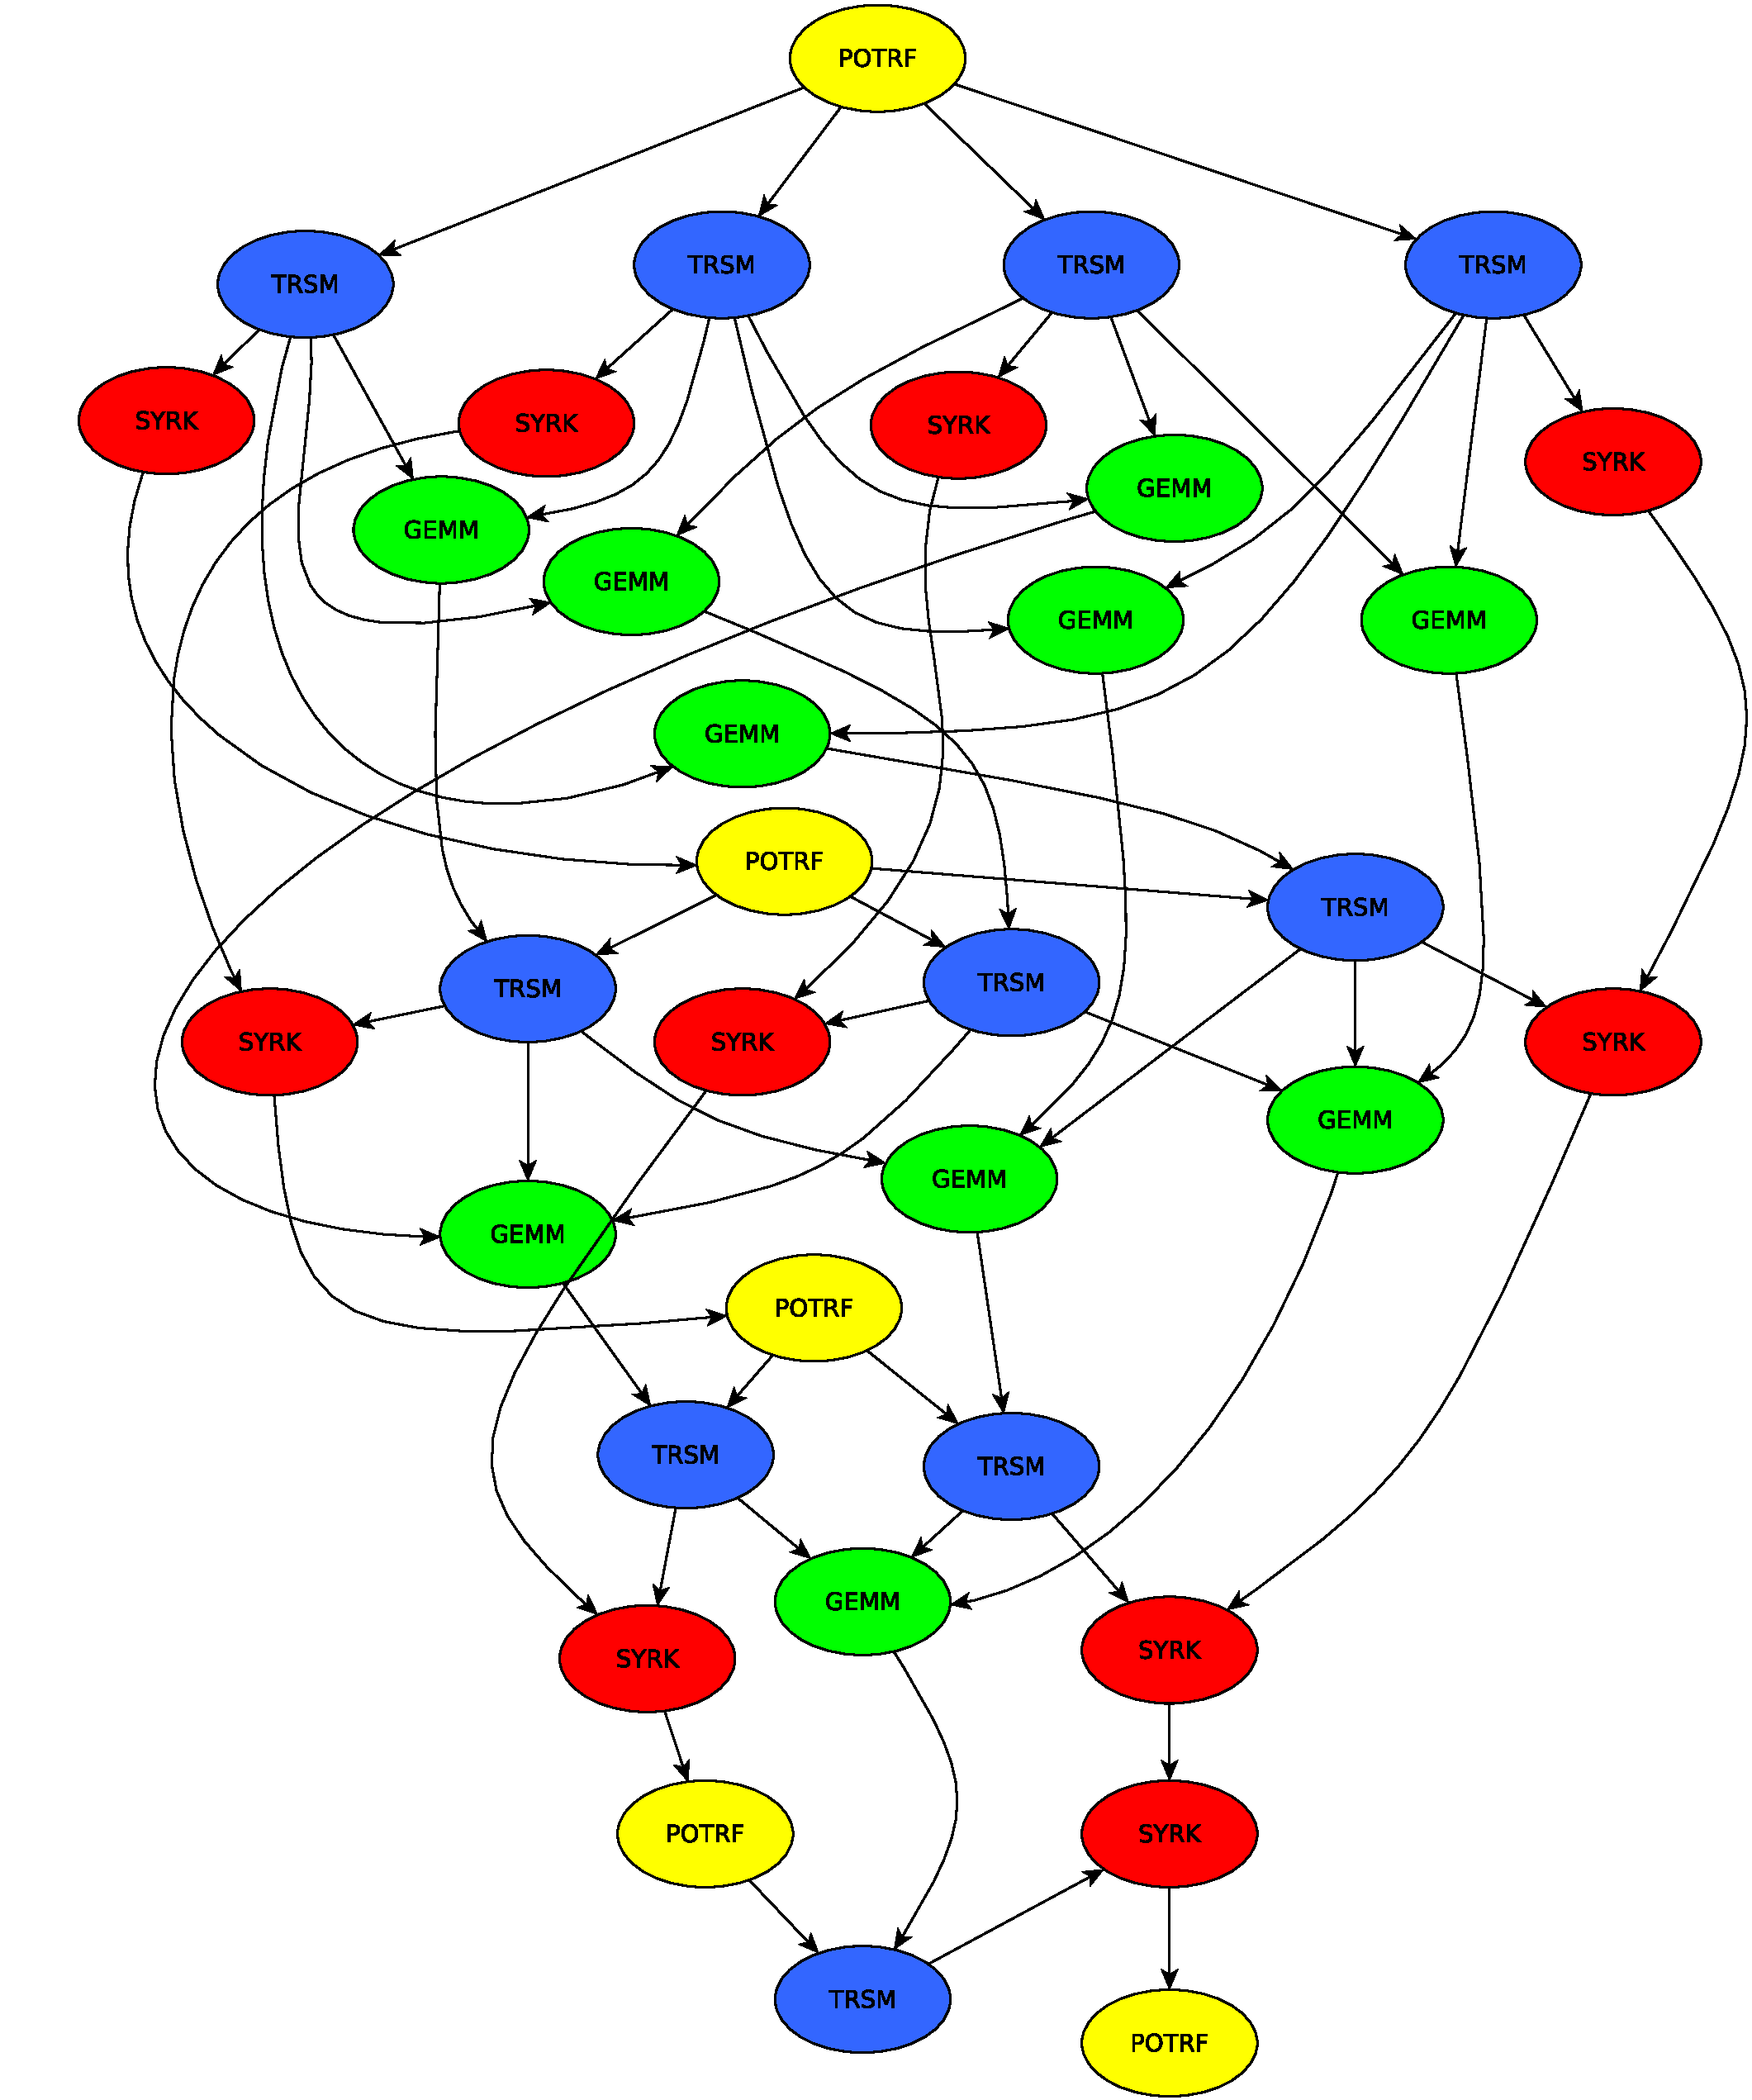
\includegraphics[width=0.7\textwidth]{cholesky-dag-5}
  \caption{DAG d'un Cholesky de largeur 5}\label{fig:contribs:apps:cholesky:dag-5}
\end{figure}

Le nombre de tâches créées au rang $k$, ainsi que le nombre d'opérations arithmétiques, ou \emph{flops}, sont résumés dans la table~\ref{tab:contribs:apps:cholesky:kernels-info}.

\begin{table}[h]
\def\arraystretch{1.5}
\centering
\begin{tabular}{|c||c|c|}\hline
  Noyau & Nombre au rang $k$ & Flops en fonction de la taille de bloc $N$~\cite{LAWN41} \\ \hline
  \potrf & 1 & $\frac{N^3}{3} + \frac{N^2}{2} + \frac{N}{6}$ \\ \hline
  \trsm & $k$ & $N^3$ \\ \hline
  \syrk & $k$ & $N^2*(N+1)$ \\ \hline
  \gemm & $\frac{k*(k-1)}{2}$ & $2*N^3$ \\ \hline
\end{tabular}
\caption{Nombre et complexité des différents noyaux}\label{tab:contribs:apps:cholesky:kernels-info}
\end{table}

Les \gemm sont donc très largement majoritaires dans l'algorithme quand la largeur de la matrice augmente, et sont également les plus intensifs en terme d'opérations.

\subsection{Observations préliminaires et limites}

La figure~\ref{fig:context:granularity} a montré qu'on pouvait observé l'impact de certains paramètres, tels que la taille de bloc ou le support exécutif, sur les performances globales.

Certains supports exécutifs permettent d'aller plus loin via un système de traces, permettant d'observer certaines caractéristiques de tâches particulières.

\begin{figure}[t!]
  \centering
  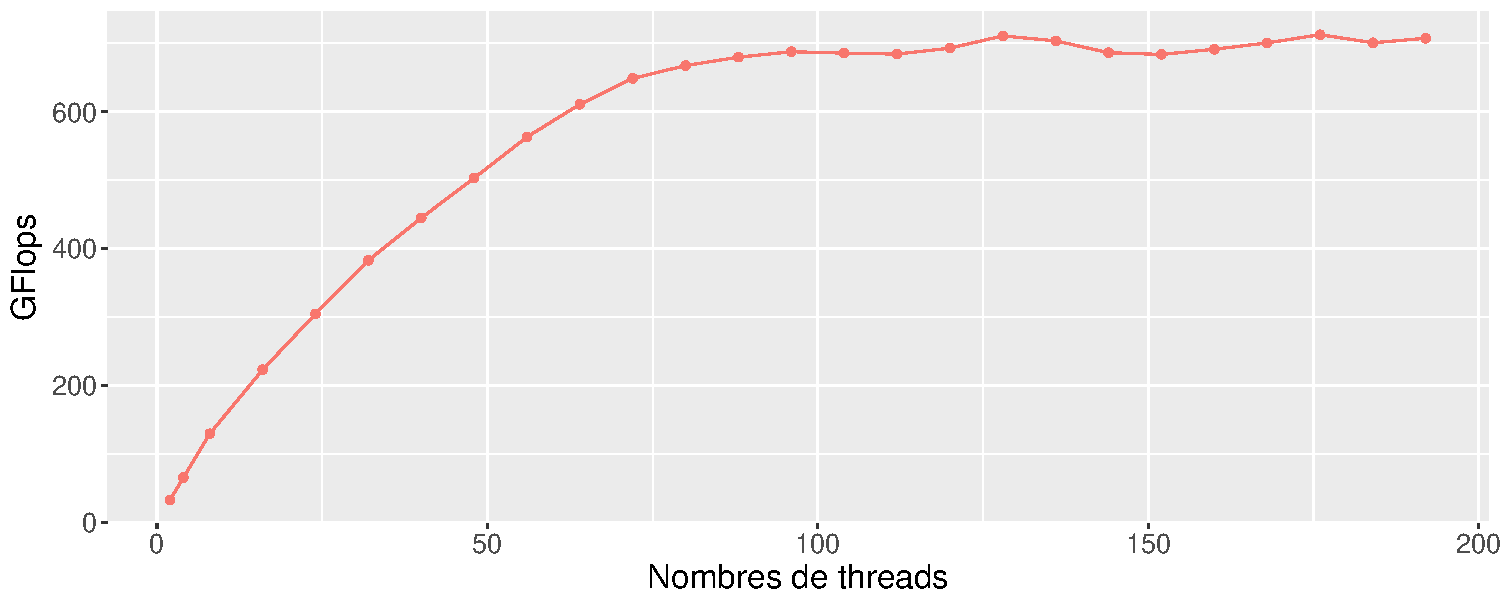
\includegraphics[width=\textwidth]{graph_evolution_cholesky_8192_224}
  \caption{Évolution des performances de Cholesky pour une taille de matrice de 8192 et une taille de bloc de 224}\label{fig:contribs:apps:cholesky:overview-8192-224}
\end{figure}

Pour illustrer cela, prenons un exemple d'évolution des performances de Cholesky en fonction du nombre de cœurs utilisés, montré sur la figure~\ref{fig:contribs:apps:cholesky:overview-8192-224}. Dans cette exemple la taille de matrice est de 8192, la taille de bloc de 224, et le support exécutif utilisé est libKOMP.

En activant le support des traces, on peut avoir plus de détails sur l'exécution individuelle de chacune des tâches.

\begin{figure}[h!]
  \centering
  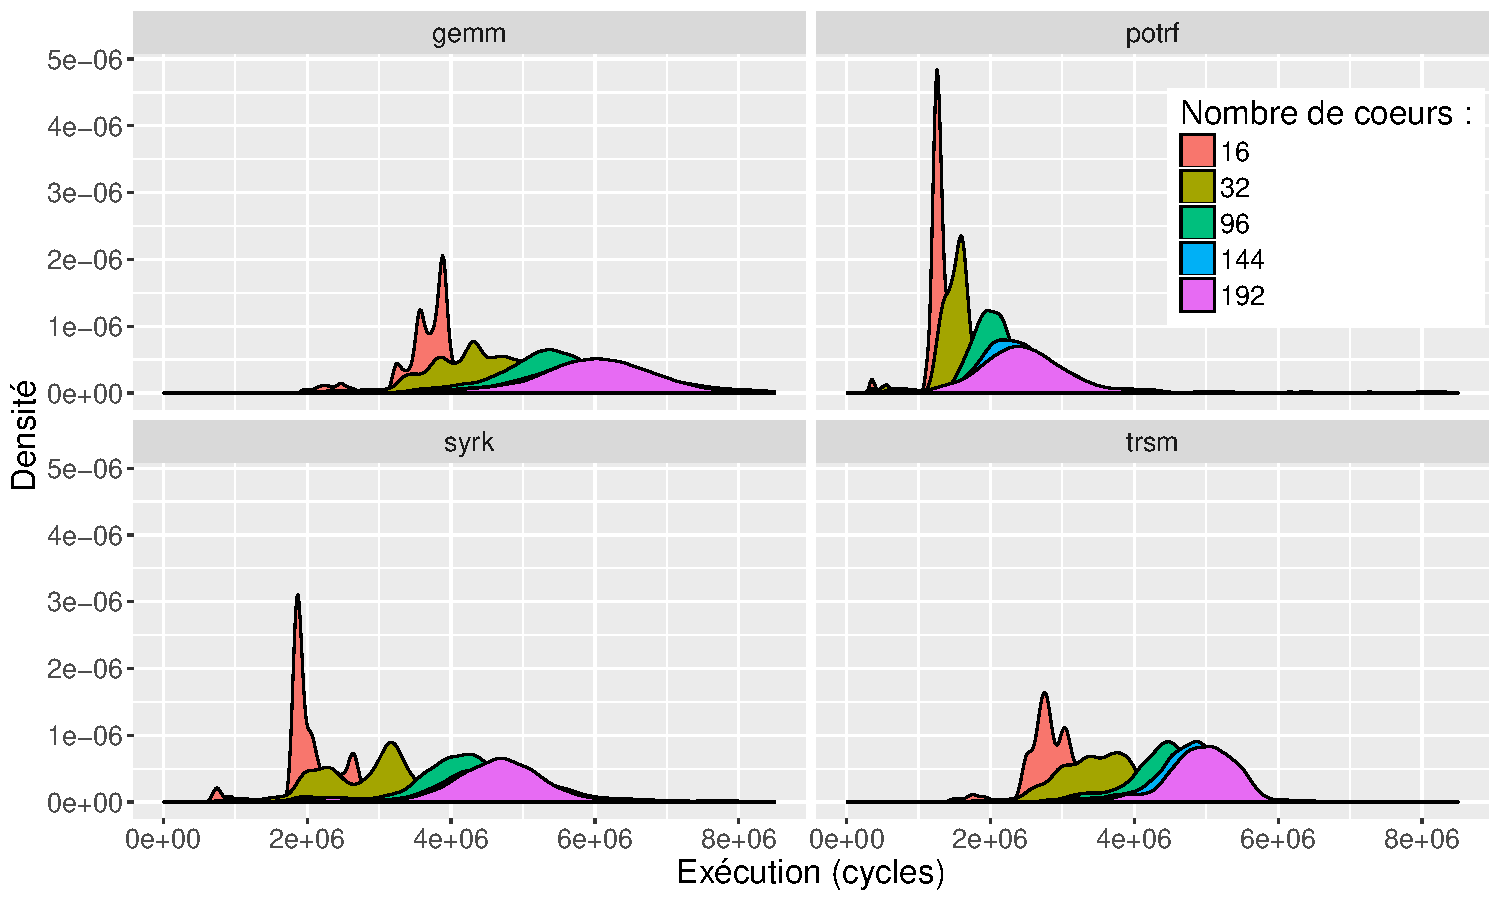
\includegraphics[width=\textwidth]{graph_distrib_overview_8192_224}
  \caption{Distribution des différents noyaux en fonction du nombre de cœurs}\label{fig:contribs:apps:cholesky:distrib-overview-8192-224}
\end{figure}

La figure~\ref{fig:contribs:apps:cholesky:distrib-overview-8192-224} montre, pour chaque type de tâche (ou \emph{noyau}), la répartition du temps d'exécution (en cycles) en fonction du nombre de cœurs.

À part pour 16 cœurs, on peut constater que la répartition est assez large~: pour un \gemm sur 192 cœurs, le nombre de cycles nécessaire pour l'exécution peut varier du simple au double !
Nous souhaiterions donc identifier d'où vient ce phénomène, afin d'éventuellement le corriger, et retomber sur un pic de performance clair et stable (comme par exemple pour la distribution des \potrf sur 16 cœurs).

Malheureusement il n'existait pas, à notre connaissance, d'outil permettant d'isoler une (ou plusieurs) tâches d'une application, et permettant de changer certains paramètres prédéfinis pouvant avoir un impact sur le temps d'exécution de la tâche.
Nous avons donc utilisé \outil dans le but de comprendre et d'analyser plus en profondeur nos observations préliminaires.

\subsection{Caractérisation détaillée des noyaux via \outil}\label{sec:contribs:apps:cholesky:carton}

L'objectif de cette section est de décrire le processus expérimental nous ayant permis d'analyser et comprendre le comportement des quatre noyaux de Cholesky~: \potrf, \trsm, \syrk, \gemm, qui a finalement abouti à des améliorations du support exécutif.
Nous allons donc aborder d'une part les types de scénarios exécutés via \outil, puis illustrer les résultats que nous avons obtenus avec des exemples significatifs.

\subsubsection{Description des scénario}

Afin d'étudier le comportement de chaque noyau impliqué dans Cholesky, nous avons définie des scénerios où ils sont exécutés avec un contrôle sur les conditions d'exécution.

Pour un noyaux donné (parmi \potrf, \trsm, \syrk, \gemm), le scénario de base est le suivant :
\begin{itemize}
  \item Allocation et initialisation des données sur un nœud précis.
  \item Exécution d'un certain nombre de répétitions du noyau choisi (par défaut 50), soit sur un cœur du même nœud, soit sur un cœur distant, pour une taille de bloc donnée.
  \item Observation de la performance en FLOPS.
\end{itemize}

Pour évaluer le comportement des noyaux en fonction de la charge de la machine, nous avons créé des scénarios exécutant plusieurs scenarios de base, de manière indépendante, et où le démarrage de l'exécution des noyaux est synchronisé.

Il y a donc plusieurs paramètres que l'on peut faire varier pour changer les conditions d'exécution~:
\begin{itemize}
  \item Le nombre de noyaux s'exécutant simultanément
  \item L'utilisation de données distantes ou locales
  \item La taille du bloc sur lequel appliquer le noyau
\end{itemize}

Les trois sections suivantes décrivent l'impact des changements de ces paramètres, et illustrent certaines caractéristiques des machines utilisées qui donnent des opportunités pour de possibles améliorations du support exécutif.

\subsubsection{Exécutions concurrentes}

\begin{figure}[ht]
  \centering
  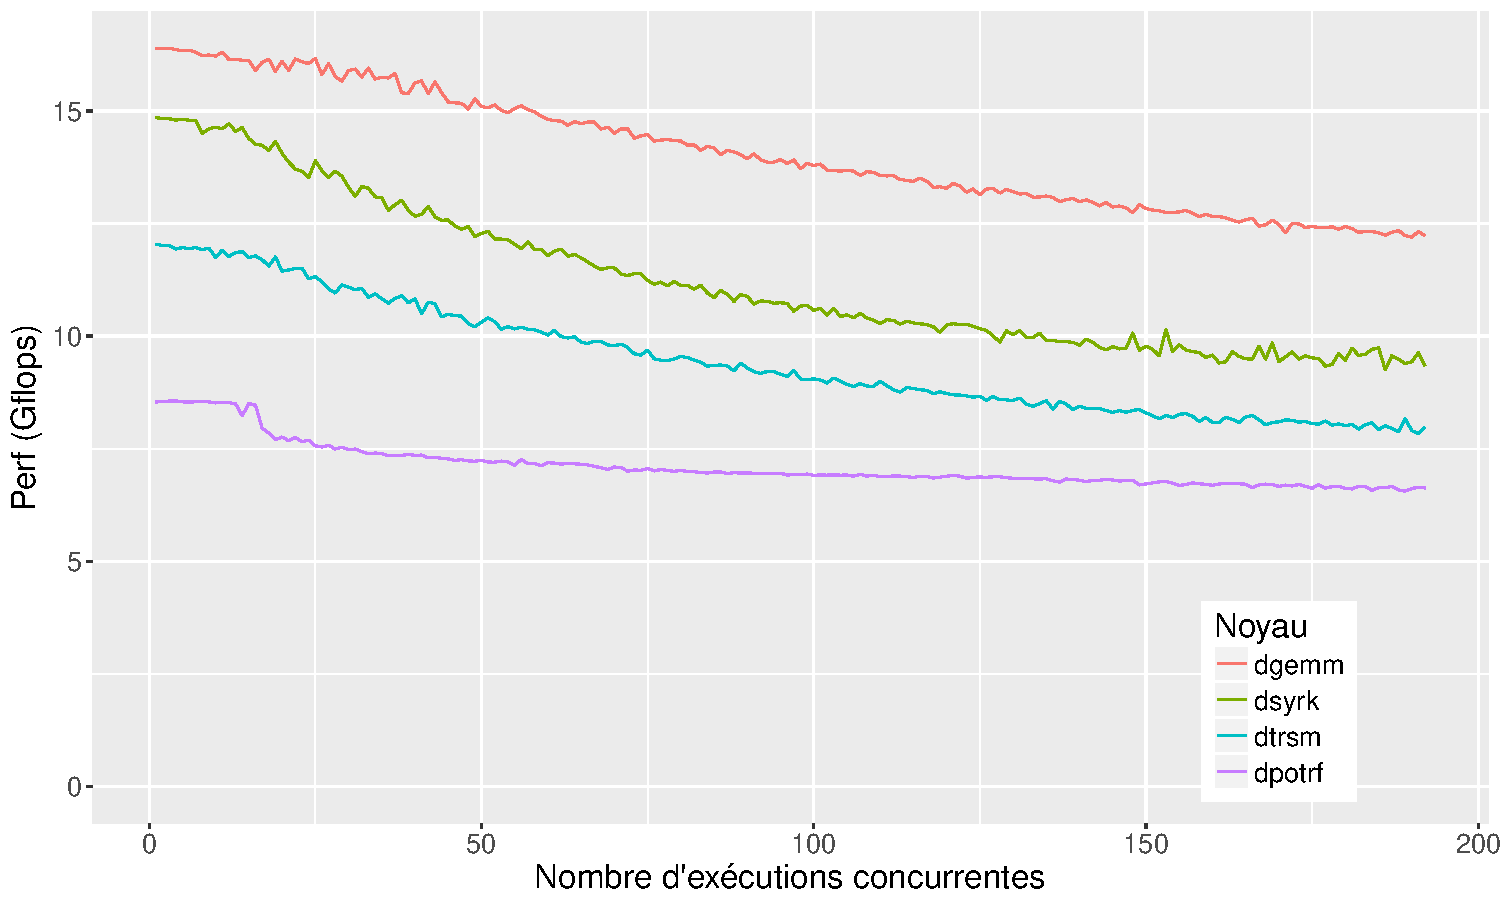
\includegraphics[width=0.95\textwidth]{kernel_256_local_idchire}
  \caption{Performances des noyaux (B=256) avec données locales sur idchire}\label{fig:contribs:apps:cholesky:perf-256-local}
\end{figure}

Afin d'évaluer l'impact de la charge de la machine, nous avons lancé des scénarios avec un nombre variable d'exécution concurrentes de chacun des noyaux. La figure~\ref{fig:contribs:apps:cholesky:perf-256-local} montre la performance moyenne (en GFlops) de chaque noyau, en fonction du nombre de cœurs exécutant des noyaux en concurrence.
Par exemple pour déterminer le point d'abscisse 150 sur la figure pour un \gemm, nous avons exécuté 50 répétitions de \gemm sur chacun des 150 premiers cœurs de la machine idchire, de manière indépendante et concurrente.
La performance moyenne pour ce point est obtenue en faisant la moyenne des performances sur l'ensemble des exécutions.
Pour ce cas la taille de bloc a été fixée à 256, avec les données allouées et initialisées localement.

Pour une taille de bloc de 256, la quantité maximale de données utilisée par l'un des noyaux (\gemm) est de 256*256*8*3 = 1.5 Mo. Avec un nœud de 8 cœurs exécutant 8 exécutions concurrentes, la quantité totale de données utilisée serait au pire de 12.58 Mo, soit environ 50\% des 20Mo de cache L3 disponible.
On pourrait donc s'attendre à ce que la performance moyenne des noyaux ne soit impactés que par des effets locaux aux nœuds.

Néanmoins les courbes montrent clairement une dégradation des performances de chaque noyaux lorsque la charge de la machine augmente.
Ce comportement a également été observé pour d'autres tailles de blocs. Sur brunch le comportement a été également observé, avec une dégradation moindre néanmoins.

\begin{todo}
  ici l'explication est toujours pas évidente : certes le nombre de messages broadcasté dépend de la quantité de données utilisées (cf lien en commentaire), mais la source principale de comm c'est les miss au L3.
  
  Là on a que des miss au L2, ça implique un write-back au L3, mais est-ce suffisant pour expliquer le phénomène ?
  %https://www.researchgate.net/profile/Daniel_Molka/publication/315703632_Performance_Analysis_of_Complex_Shared_Memory_Systems/links/58dd3cf292851cd2d3d9d5d3/Performance-Analysis-of-Complex-Shared-Memory-Systems.pdf
  %https://pdfs.semanticscholar.org/67cf/1189c859d66bac309f9438df434fb651f97a.pdf
  % sandy bridge : https://tu-dresden.de/zih/forschung/ressourcen/dateien/abgeschlossene-projekte/benchit/2014_MSPC_authors_version.pdf?lang=en
  % haswell : https://pdfs.semanticscholar.org/67cf/1189c859d66bac309f9438df434fb651f97a.pdf
\end{todo}

\subsubsection{Impact de la localité des accès}\label{sec:contribs:apps:cholesky:locality}

La section~\ref{sec:contribs:machines} a montré des différences significatives dans les temps d'accès à la mémoire locale et distante.
Nous avons donc déroulé des scénarios avec des noyaux utilisant des données distantes ou des données locales afin de pouvoir les comparer, et éventuellement déceler des comportements typiques.

\begin{figure}[t!]
  \centering
  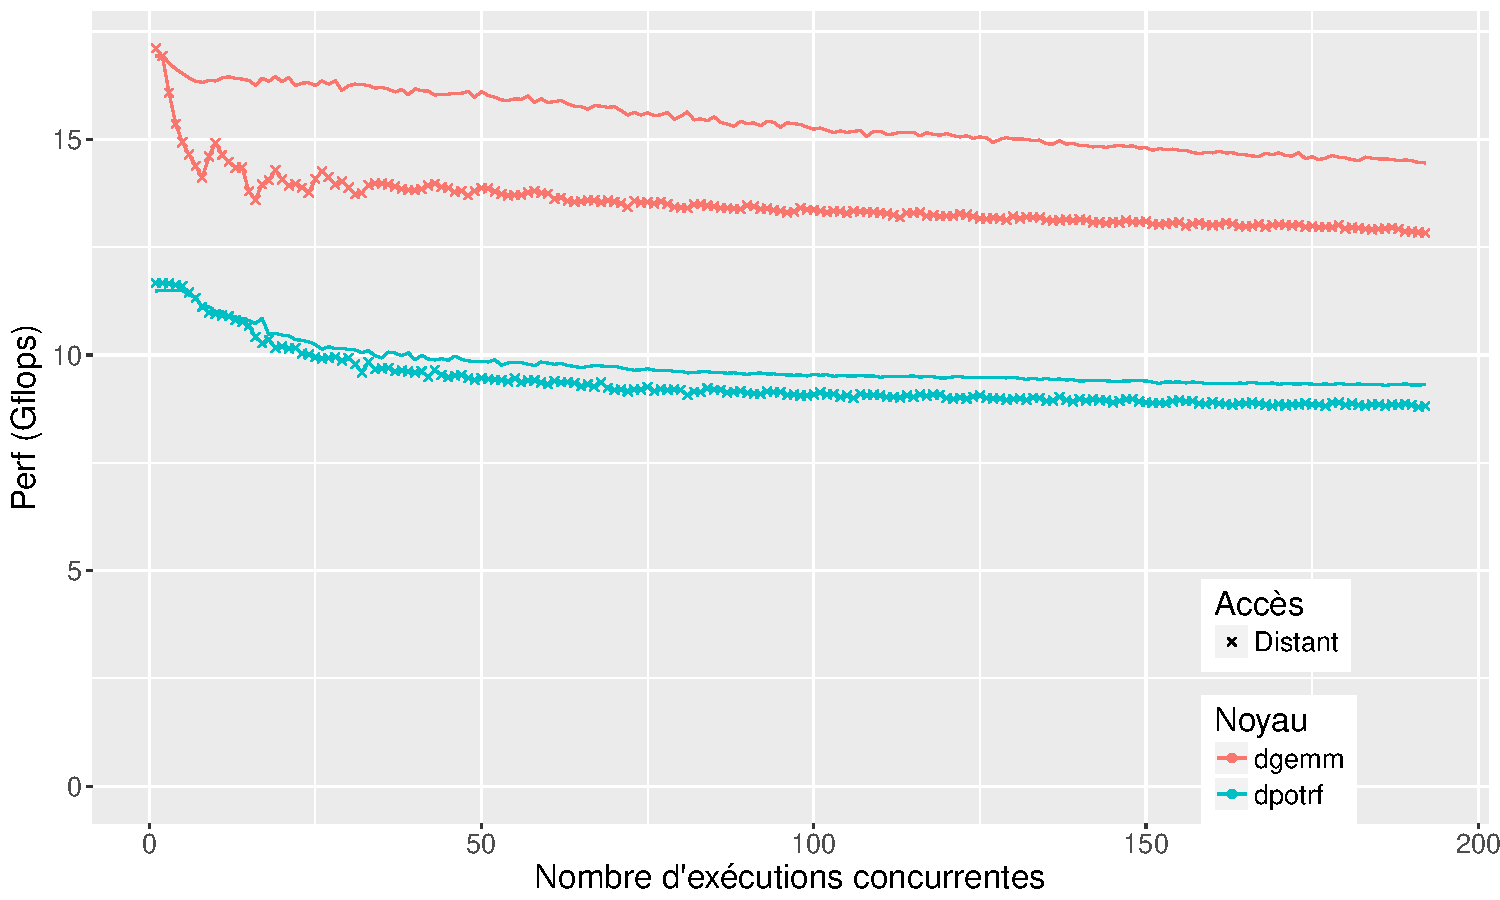
\includegraphics[width=0.95\textwidth]{kernel_512_remote_idchire}
  \caption{Performances GEMM, POTRF (B=512) avec données distantes sur idchire}\label{fig:contribs:apps:cholesky:perf-512-remote-idchire}
\end{figure}
\begin{figure}[h!]
  \centering
  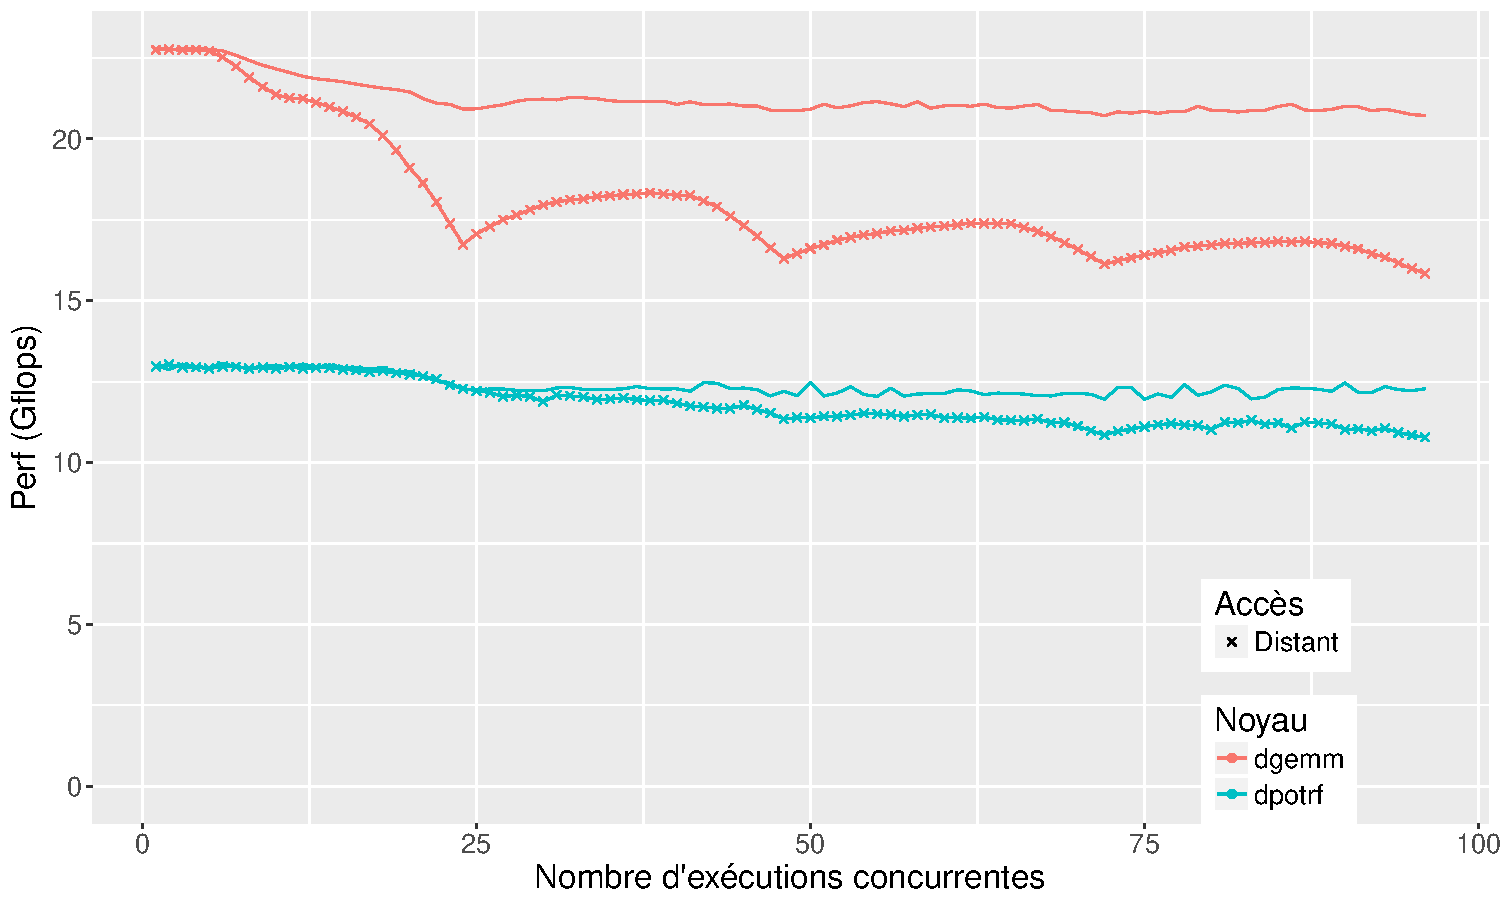
\includegraphics[width=0.95\textwidth]{kernel_512_remote_brunch}
  \caption{Performances GEMM, POTRF (B=512) avec données distantes sur brunch}\label{fig:contribs:apps:cholesky:perf-512-remote-brunch}
\end{figure}

Les figures~\ref{fig:contribs:apps:cholesky:perf-512-remote-idchire} et~\ref{fig:contribs:apps:cholesky:perf-512-remote-brunch} illustrent les performances de deux noyaux, \gemm et \potrf, effectués en concurrence sur des blocs de 512, en fonction du type d'accès, sur idchire et brunch, respectivement.

Avec une telle taille de bloc, l'ensemble des données pour tous les \potrf tient dans le cache L3, mais ce n'est pas le cas pour \gemm.
Pour les \potrf la dégradation de performances est moindre : les données tiennent dans le cache L3, il y a donc un coup pour rapatrier les données, mais une fois les données dans le cache L3 il n'y a plus besoin de faire d'accès distants.

Pour les \gemm, une utilisation de seulement quelques cœurs ne montre pas une différence de performances flagrante, en revanche le lien en sortie de nœud arrive assez vite à saturation (voir section~\ref{sec:contribs:machines:idchire:liens}), ce qui entraine une dégradation massive de performances.
À la fois pour idchire et brunch, on peut observer l'impact de la bande passante sur les performances : les courbes sont en dent de scie avec une période égale à la taille des nœuds sur chaque machine (8 sur idchire, 24 sur brunch).

Cela devient évident lorsqu'on regarde plus en détail le passage d'un nœud à un autre.
Sur la figure~\ref{fig:contribs:apps:cholesky:perf-512-remote-brunch}, la courbe pour les \gemm distants remonte progressivement entre 24 et 36 cœurs utilisés~: le fait de faire la moyenne des noyaux sur l'ensemble des cœurs cache légèrement le phénomène de saturation du lien.
En revanche ce phénomène devient évident lorsque l'on affiche la moyenne du temps d'exécution par cœurs pour certains des points de la courbe, comme illustré sur la figure~\ref{fig:contribs:apps:cholesky:distrib-load-512}.

\begin{figure}[ht]
  \centering
  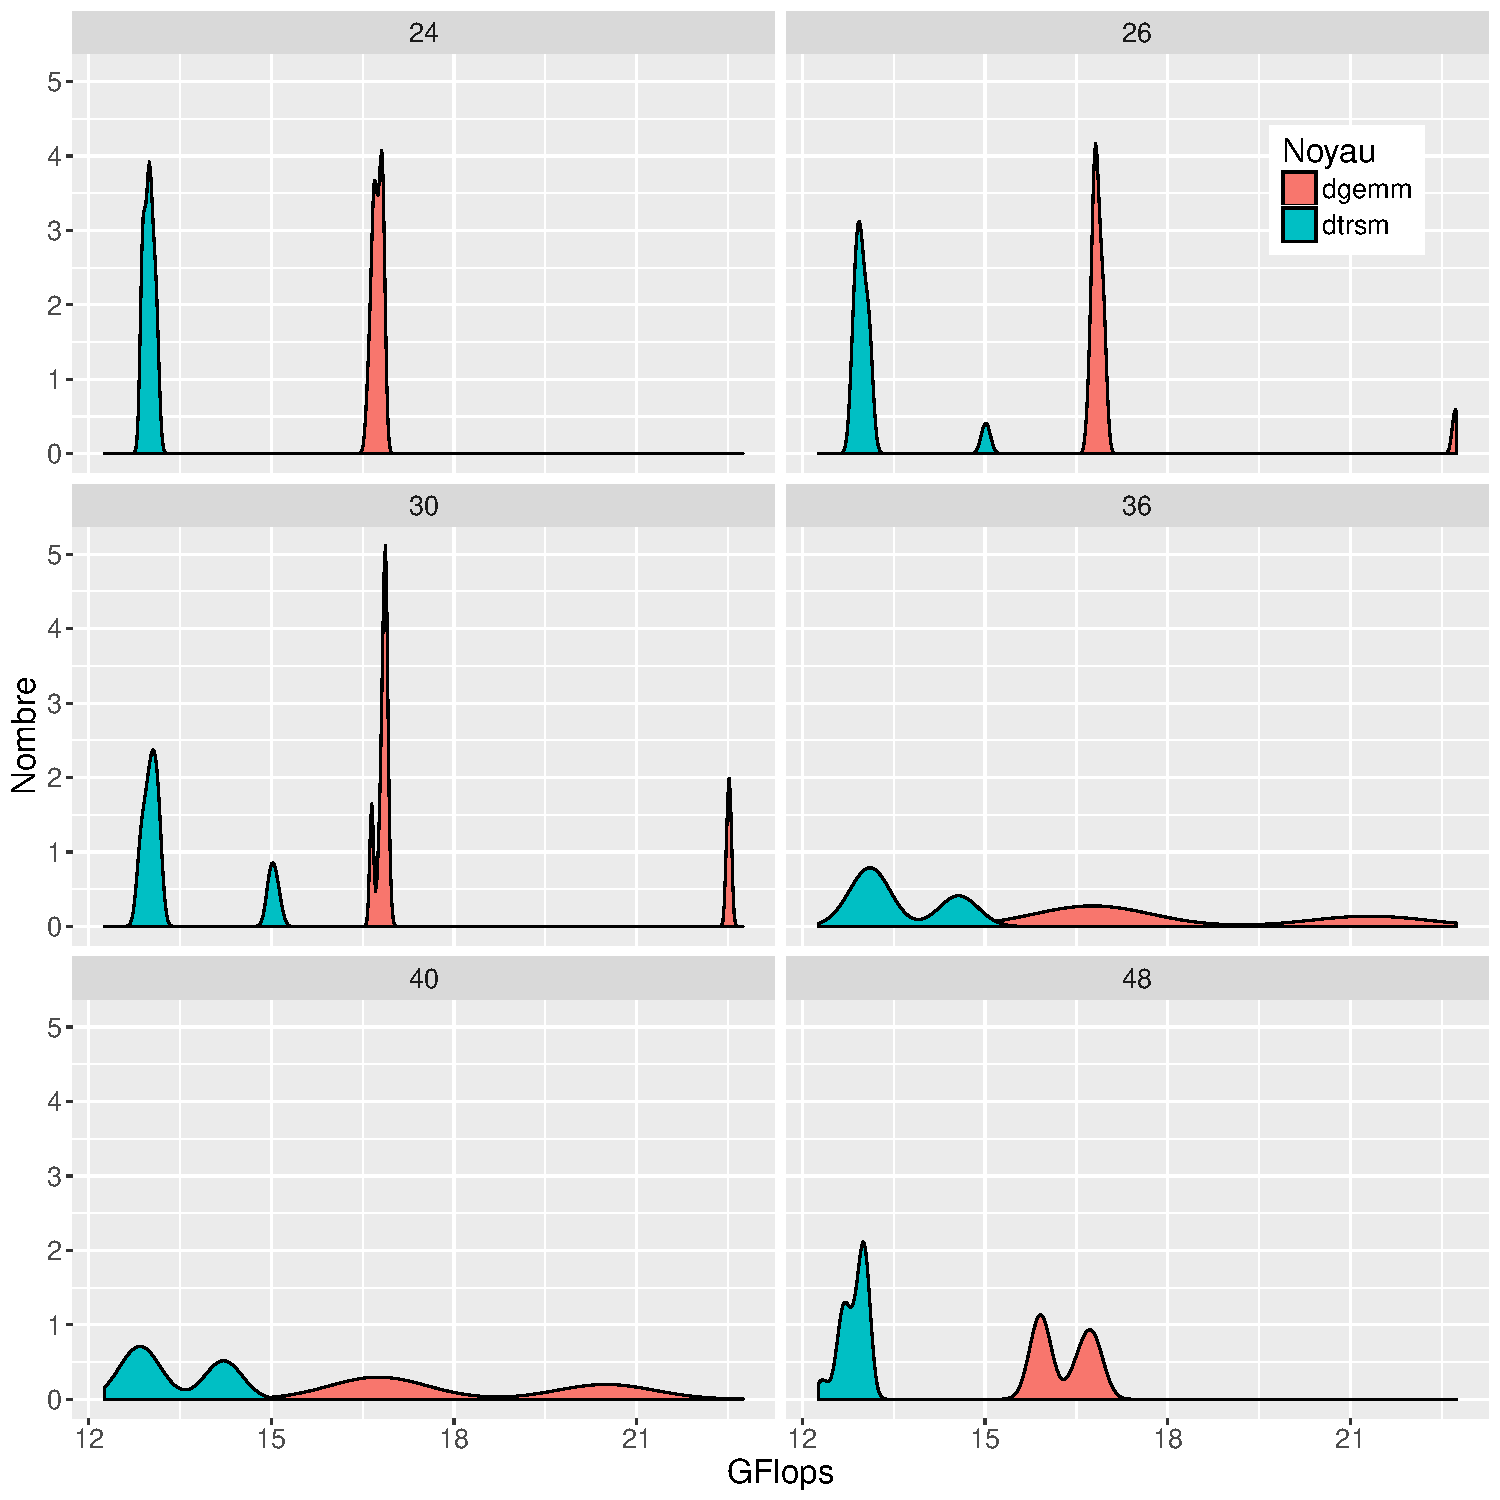
\includegraphics[width=0.95\textwidth]{illustration_load_avg}
  \caption{Distribution des performances de chaque noyau (Bloc = 512), en fonction du nombre total d'exécutions concurrentes, sur brunch}\label{fig:contribs:apps:cholesky:distrib-load-512}
\end{figure}

Le premier panneau montre la distribution des \gemm et des \potrf pour une exécution sur 24 cœurs concurrents situés sur le même nœuds.
Cette distribution montre un unique pic bien définie pour chaque noyau (environ 13 GFlops pour \potrf, et 16.5 pour \gemm).
En revanche le passage à 26 cœurs (avec donc 2 cœurs situés seuls sur un autre nœud), montre une distribution avec deux pics~: un pic important correspondant au 24 premiers cœurs, et un second pic plus petit, montrant des performances beaucoup plus grandes, pour les 2 cœurs situé sur l'autre nœud.
Les autres panneaux montrent l'évolution de ces pics pour arriver au panneau 48, où les deux nœuds sont complètement utilisés.

\begin{todo}
  Ici il y a aussi deux pics sur le panneau 48. Cela doit venir de la manière dont j'ai initialisé les accès distants : le premier nœud utilise des données du deuxième nœud, qui utilise des données du troisième nœud. Donc en pratique les liens du deuxième nœuds sont plus utilisés que ceux du premier : il doit donc un peu peiner à fournir les données nécessaires au premier nœud, ce qui expliquerait pourquoi il y a deux groupes de perf.
\end{todo}


L'impact de la localité des données est majeure dans le cas où le jeu de données manipulé par l'ensemble des cœurs ne tient pas dans le cache L3.
Étant donné que la plus grande proportion des noyaux de Cholesky manipule 2 ou 3 blocs, la dégradation de performance devrait être importante lorsque la taille de bloc dépasse environ 320.

% Note : à la fois sur brunch et idchire, chaque cœur peut utiliser environ 2.5Mo de cache L3



\subsubsection{Impact de la taille de bloc}

La figure~\ref{fig:contribs:apps:cholesky:perf-multiple-bs-idchire} montre la performance des \gemm et \potrf sur idchire en fonction de la taille de bloc et du nombre de cœurs utilisés (tous les accès sont locaux).

\begin{figure}[ht]
  \centering
  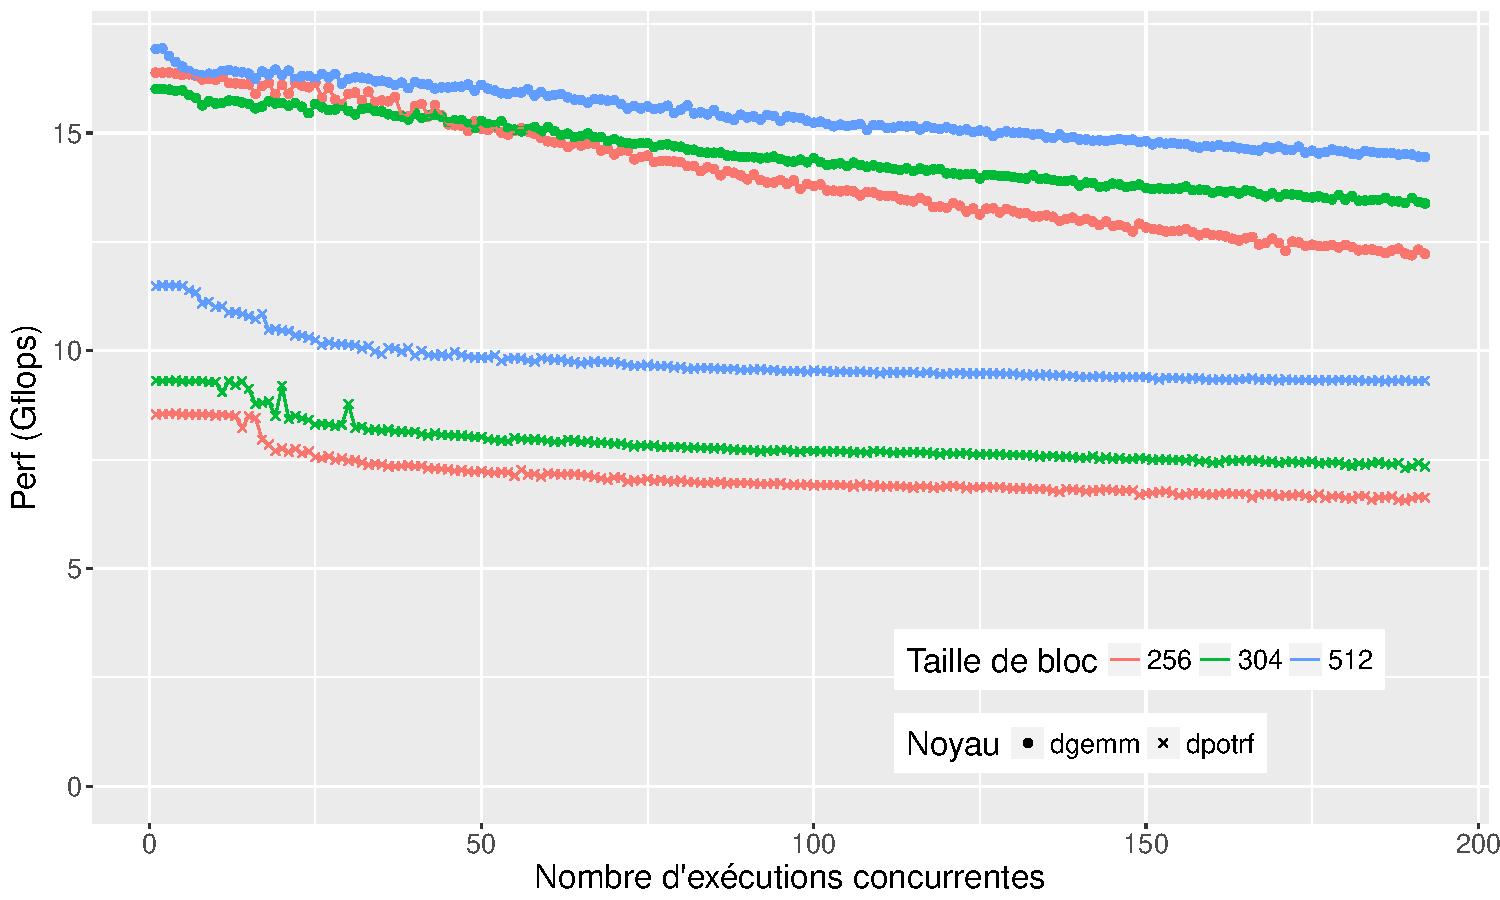
\includegraphics[width=0.95\textwidth]{kernels_multiple_bs_local_idchire}
  \caption{Performances des noyaux avec données locales sur idchire}\label{fig:contribs:apps:cholesky:perf-multiple-bs-idchire}
\end{figure}

La taille de bloc n'a pas d'impact significatif sur le phénomène observé précédemment de dégradation des performances.
Elle a bien un impact sur le niveau de performance globale de chaque noyau, mais le comportement général de chaque noyau reste le même.


\begin{todo}
  Même pas sûr de pourquoi il y a un niveau de perf différent... Je suppose que ça dépend des blas.
\end{todo}



\subsubsection{Impact de la bibliothèque BLAS}

\begin{todo}
GRAPHE : 4.3.5, dgemm/dsyrk/dtrsm faire : étude de comportement sur des paramètres représentatifs (obj : montrer l'impact des blas)
OpenBLAS, MKL, ATLAS
matter for top perf, not for overall behavior
\end{todo}

